\chapter{Related Work}
This chapter explains the previous work and concepts which led to the development of synchronization component to the KIA4SM project and it explains the synchronization algorithms available and makes a comparative study of these algorithms. 
The comparative study is based on the research work of papers which are referred here. An attempt is made to pick the best choice algorithm for the work. 

\section{Synchronization of L4 fiasco tasks}

The thesis is largely based on the work of Robert H{\"a}cker, who in his bachelor thesis \textit{ "Design of an OC-based Method for efficient Synchronization of L4 Fiasco.OC Mircrokernel Tasks"} \cite{haecker}, explains the design of a scheduler best suited scheduler for KIA4SM project and also gives comparison study of the different schedulers and synchronization methods suited for updating the task ready queue. 

He suggests Modified-Maximum-Urgency-First(MMUF) algorithm as the best choice for KIA4SM project due to the importance of safety and security in embedded systems. After comparing the synchronization algorithms the sequential lock technique has been chosen for the better control it gives. He has suggested to verify the practical implication of Read-Copy Update(RCU). At the end, he proposes a design for the existing system including aforementioned  scheduler(MMUF) and sequential locks. 

This work is an extension of H{\"a}cker's findings. However, the focus of the thesis it to develop a good synchronization method, the implementation of the scheduler is not carried out.

Some of the ideas and code knowledge is taken from the Valentin Hauner's bachelor's thesis \textit{"Extension of the Fiasco.OC microkernel with context-sensitive scheduling abilities for safety-critical applications in embedded systems"} \cite{hauner}. In this thesis he added EDF scheduling strategy. Though his thesis concentrated on using it in Genode and L4RE environment, it helped in understanding the Fiasco.OC's scheduler.

\section{Synchronization Methods} \label{rq:sync}
To do the justification to many synchronization methods are studied and are explained in this section. The synchronization categories are divided based on the methods they apply. 
The figure %TODO insert the picture 
shows the different types of synchronization methods along with examples. 

\subsection{Lock Based Algorithms}
Lock based algorithms are a simple way of enforcing the limits on access to shared resource, where there are multiple threads of execution. A lock enforces a mutual exclusion concurrency control. The area where the read or write is happening to a shared resource is called critical section. The thread has to acquire a lock before entering the critical section, only one thread can acquire this lock and whenever it leaves the critical section the thread should release the lock, so that the other threads can enter critical section.

There are many different types of lock based synchronization methods exists.

\begin{labeling}{lock}
\item[Mutex] Mutex is a synchronization primitive stands for mutual exclusion, which prevents the simultaneous access to shared resource. The thread which wants to execute in critical section has to acquire the mutex and after it leaves it has to give the mutex. 

\item[Semaphore] It's a variable used to control the common resource access between multiple processes/threads. A typical semaphore is initialized with an initial value which is equaled to the number of resources are available and the value is decremented whenever a process takes the resource. If the value of the semaphore is 0 then all the resources are empty and the thread/process has to wait. This works in the opposite way for the event management, where initial value is 0 and semaphore is increased every time an event occurs and decremented when the corresponding event is processed. A binary semaphore has only two values(0 and 1) and works similar to mutex.   

\item[Spin-lock] It's a type of lock, where the thread wants to access the critical section waits in a loop (spin) while trying to acquire the lock. The thread remains active on the CPU while no useful work is being done. Spin locks have very good advantage if the threads are blocked for shorter periods of time.
\end{labeling} 

The lock based synchronization primitives are simple, easy to implement. However, there exist a lot of disadvantages. If the programmer is not careful, deadlocks can occur and are difficult to debug. One interesting problem might arrive is priority inversion, which is defined for two threads i and j as, if J is in critical section, assign J to highest priority and when it exits critical section assign its original priority. The problem with priority inversion is, a higher thread has to wait for the lower priority thread, which is not desirable for real time systems. 

Another problem includes thread starvation, where a thread doesn't get CPU time due to long waits, which is again problem for safety critical systems, since threads should reach their deadline.
 
\subsection{Lock-Free Algorithms}

Lock Free algorithms refer to a synchronization methods where the access to critical section for all the threads is guaranteed without using the locks. Two major algorithms are discussed in the category of lock free algorithms.

\textbf{Read-Copy Update:}
Read-Copy Update (RCU) guarantees concurrent read and write operations to the same data.  It's a synchronization mechanism that was added to the Linux kernel during the 2.5 development effort that is optimized for read-mostly situations. RCU achieves scalability improvements by allowing reads to occur concurrently with updates \cite{whatisrcu}. Compared to conventional locking primitives, which ensures mutual exclusion among concurrent threads regardless of read/write operation, RCU supports concurrency between single updater and multiple readers. This is achieved in RCU by keeping multiple versions of variables and ensuring that they are not freed up until all the pre-existing readers have finished using the old copies of the variable. RCU uses three main mechanisms to achieve lock-free synchronization method which are,

\begin{labeling}{rcumethods}
\item[\textbf{Publish-Subscribe Mechanism (for insertion)}:]
Publish subscribe mechanism is a way of enforcing the compiler to execute the instructions in correct order. If a pointer is getting updated, an rcu call(rcu\_assign\_pointer())  is used to change the pointer. This can be thought of as publishing the data. This requires the readers also should wait for the update to happen to read the correct data, the dereferencing of the pointer is done by using an rcu call(rcu\_dereference()), which is further guarded by rcu read lock.

\item[\textbf{Wait For Pre-Existing RCU Readers to Complete (for deletion)}:]
The figure \ref{fig:rcu_grace} shows this mechanism in picture, where RCU's way of waiting for existing reader threads to finish. RCU introduces a grace period, where it waits on read-side critical section. The simple way to find out when the reader threads have finished the critical section is to check for the context switch of the CPU. 

\begin{figure}[h]
\centering
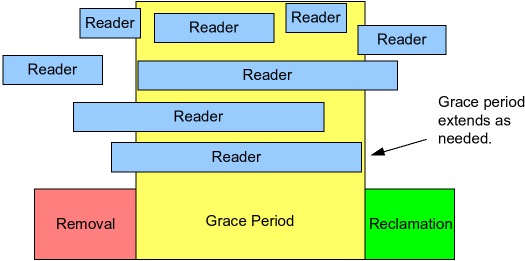
\includegraphics[width=0.7\linewidth]{figures/rcu_grace}
\caption{RCU showing the usage of grace period \cite{whatisrcu}}
\label{fig:rcu_grace}
\end{figure}

\item[\textbf{Maintain Multiple Versions of Recently Updated Objects (for readers)}]:
RCU maintains the multiple versions of the data in between removal and reclamation phases. The figure \ref{fig:rcu} shows how RCU maintains the multiple versions of data. In the linked list, B has to be removed. The first phase is changing the link from A to C, but the link from B to C still exists(removal phase). This way, if any readers were at B, they can reach C and any new readers will see only A to C. When the grace period ends, memory for B is freed(reclamation phase).

\begin{figure}[h]
\centering
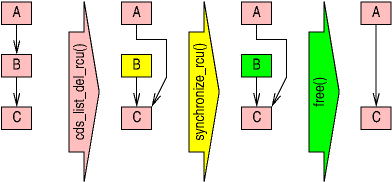
\includegraphics[width=0.7\linewidth]{figures/rcu}
\caption{Ready copy update mechanism, showing deferred destruction \cite{whatisrcu}}
\label{fig:rcu}
\end{figure}
\end{labeling}

Since the introduction of RCU, there has been lot improvements made. The research from McKenney \emph{et al.} shows that RCU can provide order-of-magnitude speedups for read-mostly data structures \cite{whatisrcu}. RCU is optimal when less than 10\% of accesses are updates over wide range of CPUs. Sarma \emph{et al.} work on making the RCU suitable for real-time systems improves on carefully RCU callbacks. They suggest three methods such as,  providing per-CPU kernel daemons to process RCU callbacks, directly invoking the RCU callback and throttling the RCU callbacks so that the limited number are invoked at a given time \cite{sarma2004making}.

\textbf{Software Transactional Memory:}
Software Transactional Memory (STM) is a concurrency control mechanism works in a similar way to database transactions by providing atomic and isolated execution for regions of code. The instructions to access shared memory are executed in a transaction, so the other threads will not see any changes when a thread is executing instructions in a transaction. At the end either the transaction is committed(if no other threads have modified the data) or aborted and the transaction is restarted. 

STM requires language extensions and compiler takes care of data versioning and conflict detection mechanisms and makes sure that the global state of the program is consistent. From GCC 4.7, STM support has been added, which makes it ideal to use in this project. The code listing shows the example transaction execution in GCC.


\begin{lstlisting}[caption={STM example code in GCC},label=sysdeploycode, style=customcpp]
void testfunc(int *x, int *y){
_transaction_atomic{
*x += *y;
}
}
\end{lstlisting}

Other nonblocking data structures which are being researched in embedded systems and other operating system groups are, 

\begin{labeling}{waitfree}
\item[\textbf{Wait-free algorithms:}] A Wait-free implementation of a concurrent data object guarantees that a thread executes in a finite number of steps, regardless of execution times of other threads  \cite{herlihy1991wait}. For example, when a higher priority thread A detects that a lower priority thread B is in critical section that A wants to enter, A lends B its priority to let B finish the execution. When B has finished, A executes in its own critical section.


\item [\textbf{Lock-free synchronization:}] It works completely without locks, this is done by using an atomic update operation like Compare-and-Swap(CAS). \textit{Critical code sections are designed such that they prepare their results out of line and then try to commit them to the pool of shared data using an atomic memory update instruction} \cite{hohmuth2001pragmatic}. It works in two steps, \textit{compare} step detects the conflict between two threads that are updating the memory location. In case of failure the whole operation is restarted. This gives deadlock free code but requires that primitives for atomic memory update operations are available.
\end{labeling}



\section{Evaluation of Synchronization techniques}

\begin{center}
\begin{tabular}{|l|l|l|p{3cm}|}
\hline 
\textbf{Criteria} & \textbf{Mutex} & \textbf{RCU} & \textbf{STM} \\ \hline

Implementation & + & - - & ++ \\ \hline

Read-speed & - - & ++ & + \\ \hline

Write-speed & - - & + & + \\ \hline

Deadlocks & - - & ++ & + \\ \hline

Overhead & + & + & - - \\ \hline

Security/Consistency & ++ & - & + \\ \hline
\end{tabular}
\captionof{table}{ Evaluation of synchronization techniques}\label{tab:lock}
\end{center}

The evaluation of these methods are according to the study of the above mentioned papers and the work of Heaker's analysis. Lock based methods and STM are easy to implement since the language constructs provide the mechanism. STM is better than locks, because with using many locks code can become unreadable while STM code has better readability \cite{pankratius2014software}. RCU is hard to implement, since the developer has to take care of providing all the read side locks, grace period handling, list operations etc.

RCU is better to use when there are multiple readers, so the read speed is very good while write-speed is still better than locks, which perform the worst in read and write speed since only one thread can access and other threads need to wait. STM's read and write is good, but only drawback it might have to read again, if the data changes in the middle of the transaction.

There is no deadlock problem in RCU, while the deadlocks are common in locks. STM also suffers from data races. RCU and locks have less overhead compared to STM. STM has to keep the logs of the transaction and has to take care to roll-back if something goes wrong. The data is consistent at all times while using locks but this is not same for RCU and STM. RCU has multiple versions of the data and STM has the logs and keeps the old data.

The recent research in STM is increasing, Ferad \emph{et al.} research suggests that implementing STM from scratch is better than trying to convert the programs from locks to STM \cite{zyulkyarov2009atomic}. The research from Victor \emph{et al.} \cite{pankratius2014software} showed that  TM is very good tool but needs C++ language refinements and better debugging support and large transactions can hurt the performance.

RCU seems a better choice for using in updating the ready queues but also it adds considerable code, given the fact that it's a embedded system. The practical approach of implementing a lock based and a lock free algorithm makes   a better case to find out the preferred method.

%\section{System Requirements} \label{foundations_cons}
%Since the system in use is a safety-critical real time system, there are certain factors to be considered in proposing a solution to the system.
%
%\begin{enumerate}
%
%\item Since the system is a safety-critical real time system, the safety becomes major criteria. The system should be in a predictable state always and is able to gracefully handle any error state.
%
%\item Any solution that is proposed should be efficient, since the used system is a embedded system. Since the system contains the less memory and processing power, the code should be simple and efficient.
%
%\item The utilization of the CPU should be intelligent to ensure that the all threads reach their deadline, since the computed value of no use once the deadline has passed. This requires a effective scheduling strategy to be used. 
%
%\end{enumerate}